
\section{Week 9: the evidence contract}
\textbf{Meeting: Monday, 2 November 2026, 14:00--17:00.} This week allocates 60 minutes to explanation and 120 minutes to practice. H1 contains 45 minutes of explanation and 15 minutes of hand calculation; H2 contains 15 minutes of explanation and 45 minutes of guided computing; H3 is a 60-minute lab. There are eight core exercises and two optional challenges. They are in-class formative practice, not new weekly graded homework.

By the end, students should distinguish aggregate and subgroup error, diagnose a missing feature term, distinguish input shift from target-mechanism shift, interpret a standardized model in original feature coordinates, and replay a result from an exact CSV. Prerequisites are regression, held-out evaluation, MAE, and Python arrays.

\subsection{A result is conditional}
Let $f$ be a fixed fitted predictor and $L$ a declared loss. Population risk is
\[
 R_P(f)=\mathbb{E}_{(X,Y)\sim P}[L(Y,f(X))].
\]
A finite test average estimates this risk under sampling assumptions; it is not the population expectation itself. A score on population $P$ does not automatically establish the same score on another population $Q$. Name the population, split, units, loss, group counts and model version whenever making a performance claim. A successful software execution is not equivalent to validation of a deployed engineering system.

\section{Residuals, metrics, and mixtures}
We use the sign convention $e_i=\widehat y_i-y_i$. Positive residuals mean overprediction, negative residuals mean underprediction. Some references reverse this convention; the plots and interpretation must remain consistent.
\[
 \operatorname{MAE}=\frac1n\sum_i|e_i|,\qquad
 \operatorname{RMSE}=\sqrt{\frac1n\sum_i e_i^2}.
\]
Both metrics have response units. MSE has squared response units. RMSE is at least MAE for the same equally weighted rows, but neither metric is universally the correct decision criterion. Declare the loss and the costs it represents before selecting a winner.

\subsection{A complete subgroup calculation}
For disjoint exhaustive groups $g$ with $n_g$ observations and $w_g=n_g/n$,
\[
 \operatorname{MAE}=\sum_gw_g\operatorname{MAE}_g,\qquad
 \operatorname{RMSE}=\sqrt{\sum_gw_g\operatorname{RMSE}_g^2}.
\]
The first identity follows by partitioning the absolute-error sum; the second follows by partitioning the squared-error sum. Directly averaging subgroup RMSEs is generally wrong.

Consider 90 observations with absolute error 1 and 10 with absolute error 10. Total absolute error is $90+100=190$; overall MAE is 1.9. The subgroup MAEs are 1 and 10. Changing only the mixture to 75/25 gives $(75+250)/100=3.25$. Neither subgroup improved or deteriorated. An aggregate dashboard can therefore change with population composition.

Report counts alongside all slice metrics. An empty group has no defined empirical mean, not an error of zero. A group of two and a group of two hundred can share the same mean but supply very different amounts of evidence. Repeatedly searching final-test boundaries for a favourable score is exploratory analysis, not independent confirmation.

\subsection{An outlier worked example}
For residuals $[0.1,-0.1,0.2,-0.2]$, $\sum|e_i|=0.6$ and $\sum e_i^2=0.1$. Thus MAE is $0.15$ and RMSE is $\sqrt{0.025}\approx0.1581$. Appending a fifth residual of 3 changes the sums to 3.6 and 9.1. With $n=5$, MAE becomes 0.72 and RMSE becomes $\sqrt{1.82}\approx1.3491$. The large squared contribution explains the stronger response of RMSE. Remember that appending changes the denominator too.

\section{Why the known generator is useful}
The teaching dataset has 500 independent synthetic observations:
\[
 X_0,X_1,X_2\overset{\mathrm{iid}}\sim\mathcal N(0,1),\quad
 \epsilon\sim\mathcal N(0,0.2^2),\quad
 Y=2X_0+X_1^2+\epsilon.
\]
Inputs are dimensionless synthetic numbers, not measured physical quantities. The response has synthetic response units. $X_2$ is a negative control. The known relation is stipulated for teaching; we have not discovered a physical law.

Two candidates are declared before final evaluation. The first applies training-fitted standardization and Ridge regression to $[x_0,x_1,x_2]$. The second adds the fixed feature $x_1^2$, then applies training-fitted standardization and Ridge. Both use $\alpha=1$ and an SVD solver. The linear candidate cannot exactly represent a squared term. Standardization alone is affine and cannot manufacture that missing basis function.

\subsection{Split, select, then evaluate}
Reserve 350 training rows, 75 validation rows and 75 test rows. Store every row ID and its split. Check all three pairwise intersections are empty and the union contains exactly all 500 rows. Random splitting is appropriate here because the observations are independent synthetic draws. Repeated machines or temporal records require grouped or chronological evaluation instead.

Fit scalers and regression parameters on training rows only. Select the candidate with the lowest validation MAE; exact ties favour the linear candidate. Freeze this choice before opening final test evidence. Report the predeclared comparison of both candidates, but do not change the selected winner based on final-test performance. This protocol retains training-only fits; it does not silently refit on training plus validation.

\subsection{What a residual shape explains}
A simple noise-free linear approximation uses $2x_0+1$ in place of $2x_0+x_1^2$. Its residual is $1-x_1^2$, giving negative tails. The actual fitted model includes noise, finite-sample coefficients and regularization, so its scatter need not equal this exact curve. In real observational data, a curved residual is a diagnostic clue, not proof of a particular physical cause.

\begin{figure}[htbp]\centering
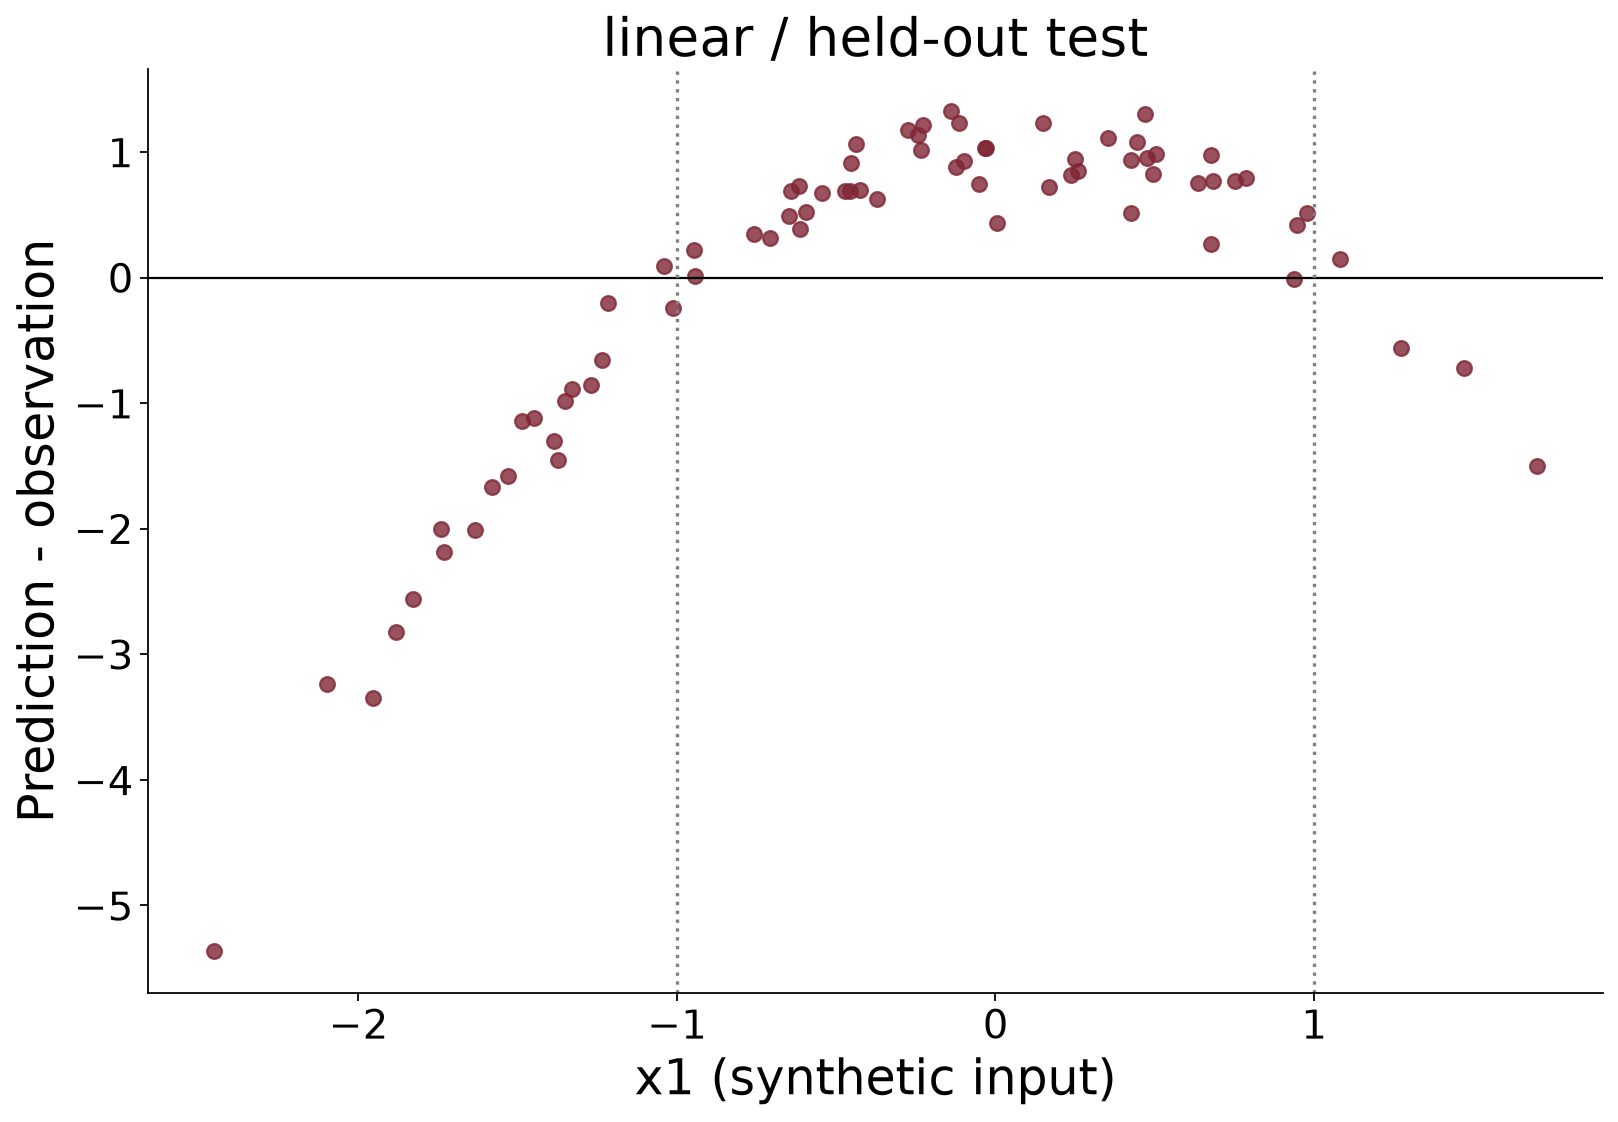
\includegraphics[width=.48\textwidth]{figures/week09/w09-linear-residuals.png}\hfill
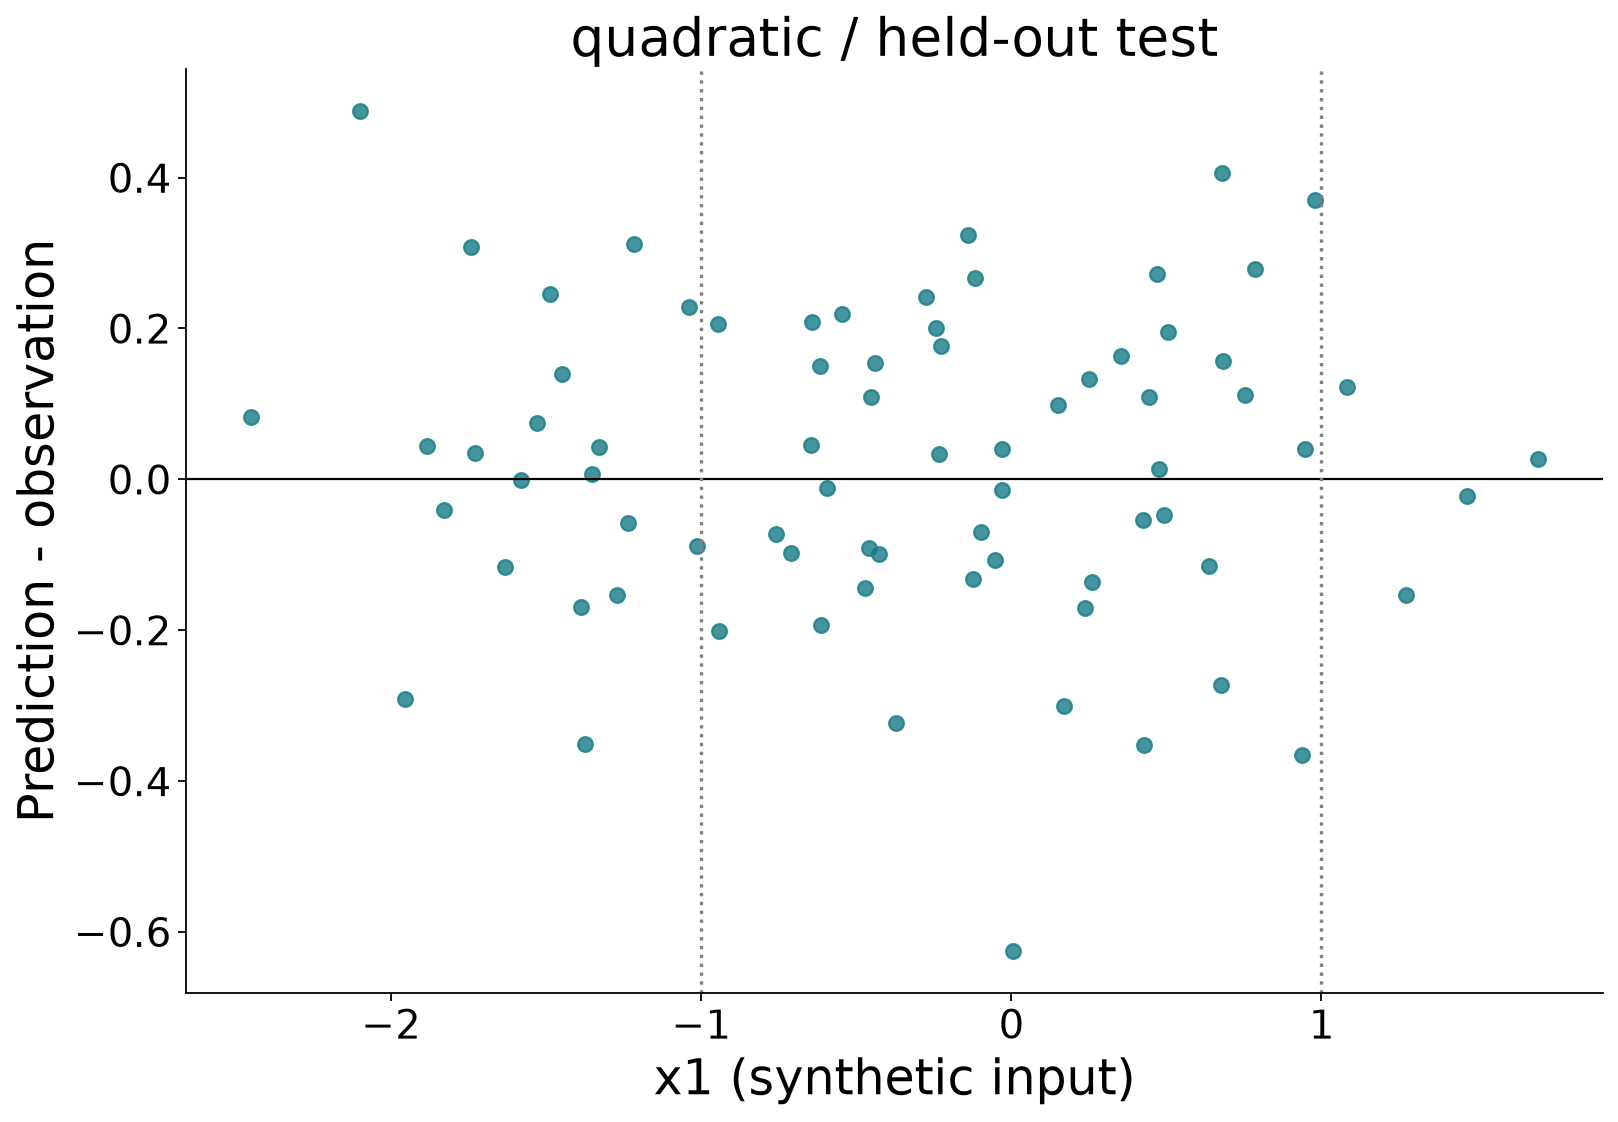
\includegraphics[width=.48\textwidth]{figures/week09/w09-quadratic-residuals.png}
\caption{Actual synthetic reference test residuals. Sign: prediction minus observation. The panels have independently chosen vertical scales; compare numerical magnitudes, not just occupied plot area.}\end{figure}

\section{Two kinds of change}
\subsection{Covariate shift}
Under covariate shift, $P(X)$ changes while the stipulated $P(Y\mid X)$ remains fixed. The lab draws a separate 150-row base population and noise vector. For severity $s\in\{1,1.5,2.5\}$, copy the base observations, multiply only $x_1$ by $s$, and recompute $y=2x_0+x_1^2+\epsilon$ using the same noise. Keep $x_0$, $x_2$, fitted parameters and candidate selection unchanged. Pairing conditions makes comparisons less contaminated by new random draws; it does not remove all uncertainty.

An exactly represented known function may respond much better than a misspecified linear candidate in this experiment. Do not infer that all distribution shifts necessarily worsen every model, or that a particular finite-sample error ratio is universal.

\subsection{An analytic stress test is not the fitted experiment}
For the fixed toy predictor $\widehat y=0$ and target $y=x^2$, absolute residual equals $x^2$. For $X\sim\mathcal N(0,\sigma^2)$, population MAE is $\sigma^2$. A different toy uses 101 endpoint-inclusive, equally spaced points on $[-L,L]$. Its grid MAE is $0.34L^2$, giving 0.34 for $L=1$ and 3.06 for $L=3$. The exact ratio of 9 follows from scaling the same normalized grid. The finite-grid mean differs from the continuous uniform expectation $L^2/3$. Neither toy is the fitted Ridge experiment.

\begin{figure}[htbp]\centering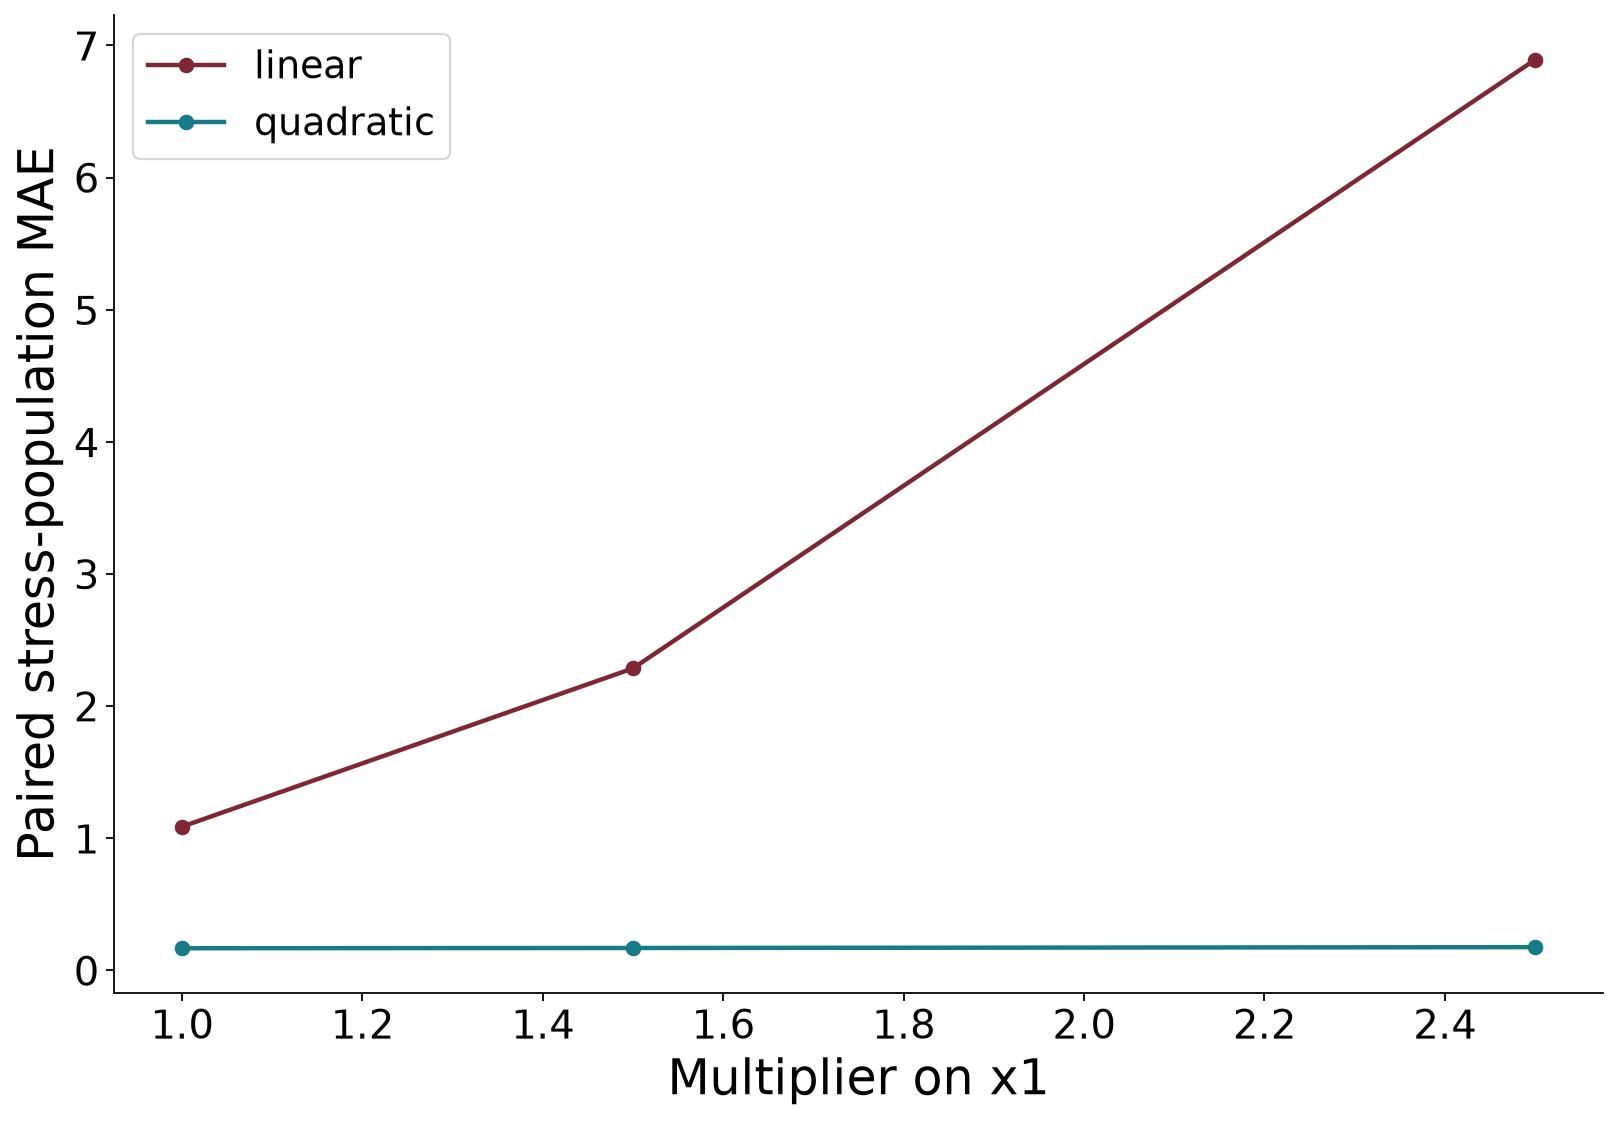
\includegraphics[width=.78\textwidth]{figures/week09/w09-stress-mae.png}
\caption{Actual errors of frozen fitted candidates on paired synthetic stress populations. These are specified teaching conditions, not external deployment validation.}\end{figure}

\subsection{Concept shift can hide from input checks}
Keep exactly the same test inputs, noise and model predictions, but define changed outcomes $y'=-2x_0+x_1^2+\epsilon$. Now the conditional target relation changes while the input rows and histograms remain identical. An input-only monitor cannot detect this constructed change. Comparing predictions with the changed outcomes can expose changed error. In a real system, outcome availability, delay and selection must also be considered.

An input-range flag is not an error label. Observed training min/max describe a finite sample. Gaussian support is unbounded, so being outside the observed range does not imply being outside mathematical support. Changed inputs motivate investigation; outcomes or another justified procedure are needed to assess prediction error.

\section{Interpretability as a checked equation}
For one standardized feature, $z=(x-\mu)/s$ and model term $\beta z$ give a raw coefficient $\beta/s$. For all transformed features,
\[
 \beta_j^{\mathrm{raw}}=\beta_j/s_j,\qquad
 b^{\mathrm{raw}}=b-\sum_j\beta_j\mu_j/s_j.
\]
Use the scaler fitted after the fixed basis expansion. Reconstruct the complete raw-coordinate prediction and assert agreement with the pipeline. Task 5 perturbs $x_0$ by $0.5$. Its predicted difference is exactly $0.5\beta_{x_0}^{\mathrm{raw}}$ for these models. This describes the fitted function conditional on its representation; it is not evidence of real-world causation.

The optional symmetry check flips $x_1$. The squared feature is even, but a fitted linear $x_1$ term can produce $f(-x_1)-f(x_1)=-2\beta_{x_1}^{\mathrm{raw}}x_1$. Noise and regularization do not guarantee that the fitted odd coefficient is exactly zero.

\section{Uncertainty and evidence identity}
\subsection{The bootstrap is conditional}
The notebook resamples absolute test residuals within a slice, computes 300 resampled means, and reports the 2.5th and 97.5th percentiles. This is a descriptive fixed-model interval under an IID-within-slice assumption. It does not cover all training, selection or future-shift uncertainty. For fewer than two observations, no interval is reported. Narrowness is not a safety certificate.

\subsection{Freeze and replay}
Export an exact CSV containing row ID, split, features and target; compute its SHA-256. Retain configuration, package versions, candidate definitions, selected winner, metrics, counts, predictions and original-space coefficients. A hash identifies bytes relative to a recorded digest; it does not validate a scientific claim or labels.

Load the frozen CSV, recover saved training and test membership, clone the already selected candidate, fit on its training rows, and compare its test predictions with the original vector. The notebook uses absolute and relative tolerances of $10^{-10}$. Record the actual maximum difference. Agreement under this recorded environment is a reproducibility result, not a guarantee of bitwise identity on every platform.

Task 7 appends a blank line to a copy of the CSV. Its bytes and checksum change while the parser recovers the same 500 nonempty records. The original remains unchanged. This is a concrete counterexample to confusing byte identity with semantic equality or scientific validity.

\section{Eight core exercises and two optional challenges}
Each core exercise requires a prediction written before execution and an explanation afterward. Record the actual observation, an equation or mechanism, and a stopping check. Work in pairs and alternate driver and reviewer. The full exercise notebook includes the walkthrough, so it can be opened on its own.
\begin{enumerate}
\item \textbf{Mixture calculation (H1):} derive 1.9 and 3.25; show weights and subgroup counts. Stop when both subgroup losses and population change are explicit.
\item \textbf{Slice sensitivity (H2):} compare boundaries $|x_1|=0.5,1,1.5$ on frozen test predictions. Report both group counts and MAEs; each pair must sum to 75. Label this exploratory, not model selection.
\item \textbf{Grid stress (H1):} derive the factor of 9 before running the 101-point grid. Explain the distinction from a Gaussian population.
\item \textbf{Outlier metrics (H1):} show both intermediate sums and denominators before checking MAE/RMSE with code.
\item \textbf{Function perturbation (H3):} add 0.5 to $x_0$ only and verify the raw-coefficient prediction difference within tolerance.
\item \textbf{Paired extension (H3):} predeclare scale 2.0, reuse base stress inputs and noise, and compare both actual candidate metrics. Assert parameter snapshots unchanged. Preserve the original reference conditions separately.
\item \textbf{Byte identity (H3):} alter a copy by one blank line, verify different hash and identical parsed rows, and confirm the original hash unchanged.
\item \textbf{Concept shift (H3):} change the stipulated target coefficient of $x_0$ from 2 to $-2$, leaving inputs and predictions fixed. Compare actual errors and explain the input-monitor blind spot.
\end{enumerate}
Optional challenge A checks fitted-function symmetry under $x_1\mapsto-x_1$. Optional challenge B multiplies served $x_0$ by 100 without changing intended targets, then decodes by dividing by 100 and verifies restoration of original predictions. These dimensionless synthetic values illustrate an encoding mismatch, not a measured physical unit conversion. Optional work is not required for core completion.

\subsection{The result card and export}
The 19 required response fields comprise eight predictions, eight explanations, one controlled change, one limitation and an AI-use/checking disclosure (or ``none''). Missing responses produce status \texttt{draft}; nonempty fields produce \texttt{ready for peer discussion}, not a correctness grade. Rerun only the final export after editing responses: rerunning initialization would erase them.

Retain both the reference ZIP and the exercise ZIP. The exercise record contains observations and completeness status. Download before closing a free Colab runtime. No paid AI, GPU, external data or API key is required. AI may assist with a hypothesis or code explanation, but every claimed number must come from actual execution. Record material assistance and checks.

\section{Reference execution and its limits}
The accompanying source notebooks were executed from top to bottom in fresh isolated CPU Jupyter kernels on 19 October 2026. This is not a claim of execution in the Google Colab browser. Students must record their own environment and results. Model training, held-out evaluation, 14 figure exports, CSV replay, ZIP integrity, all core tasks, optional branches, and draft/completed export branches were checked locally. Public student notebooks retain blank outputs and responses.

\begin{center}\begin{tabular}{lrrr}\toprule Candidate & Test n & Test MAE & Test RMSE \\ \midrule
linear & 75 & 1.031530 & 1.319474 \\
quadratic & 75 & 0.164319 & 0.205100 \\
\bottomrule\end{tabular}\end{center}

\textbf{Evidence identity (SHA-256):}\par\noindent{\small\texttt{994925f73576edc48f352b4b7300221eda8ed4c117e4f3615382579adf9411ab}}\par This hash identifies the exact reference CSV. The generated relation and all evaluation populations are synthetic; these outputs do not establish performance on real machines, financial data, or a deployed service.

\section{Summary and next dependency}
Always pair averages with populations and group counts. Use residuals to motivate explicit hypotheses. Distinguish a changed input distribution from a changed target mechanism. Freeze fitted models during stress evaluation, interpret coefficients in the correct coordinates, and replay exact inputs before claiming reproducibility. Week 10 turns this evidence trail into a compact workflow demonstration. Written and oral examination requirements remain unchanged.

\section{Further reading}
\begin{itemize}
\item Google Machine Learning Crash Course, monitoring pipelines: \href{https://developers.google.com/machine-learning/crash-course/production-ml-systems/monitoring}{Monitoring pipelines documentation}.
\item scikit-learn, common pitfalls and leakage-safe preprocessing: \href{https://scikit-learn.org/stable/common_pitfalls.html}{Common pitfalls documentation}.
\item scikit-learn, regression evaluation: \href{https://scikit-learn.org/stable/modules/model_evaluation.html}{Regression evaluation documentation}.
\item Koh et al., WILDS (2021), natural distribution-shift benchmarks: \href{https://proceedings.mlr.press/v139/koh21a.html}{WILDS paper and benchmark description}. This is contextual research, not the dataset used in this lab.
\end{itemize}
